\chapter{Parameter Minimization using the Levenberg-Marquardt algorithm}
\emph{Do some fitting}
\section{Introduction}
The Levenberg-Marquardt plugin is used to fit a SBML models parameters to experimental data. 

The current implementation is based on the lmfit C library by Joachim Wuttke. See footnote\footnote{The package lmfit is distributed under the FreeBSD License:

--
  Copyright (c) 2013 Joachim Wuttke All rights reserved.
--} for license disclosure.

The plugin has numerous properties to allow the user full control over the internal fitting engine, as well as 
access to generated fitted data after a minimization session. 

Plugin properties are documented in the next section.

\begin{landscape}
\section{Plugin Properties}
Available properties in the Levenberg-Marquardt plugin are listed in the table below.

%\begin{table}[ht]
\centering % used for centering table
\begin{longtable}{p{4cm} l p{3cm}  p{10cm}} % centered columns 

Parameter Name & Data Type & Default Value  & Description \\ [0.5ex] % inserts table 
%heading
\hline % inserts single horizontal line
SBML                            &   string              & N/A    &   SBML document as a string. Model to be used in the fitting. \\
ExperimentalData   				&	roadRunnerData 		& N/A    &   Input data.  \\
FittedData      				& 	roadRunnerData    	& N/A    &   Output data. \\
Residuals     					& 	roadRunnerData    	& N/A    &   Residuals data.  \\
InputParameterList 				&	listOfParameters    & N/A    &   Parameters to fit. \\
OutputParameterList 			&   listOfParameters 	& N/A    &   List of fitted parameters. \\
Experimental\-DataSelectionList & 	stringList			& N/A    &   Species selection list for experimental data. \\
FittedDataSelectionList     	& 	stringList			& N/A    &   Selection list for model data. \\
Norm							&	double				& N/A    &   Norm of fitting. An estimate of goodness of fit. \\
NrOfIter                        &   int                 & N/A    &   Number of iterations. \\[12pt]
\\[2pt]                                                               
\multicolumn{4}{p{19cm}}{The following properties are used internally by the fitting engine. They are preset with default values. Depending on the minimization problem at hand, they may need to be tweaked. } \\[12pt]
\hline %inserts single line                                           
\\[2pt]                                                               
ftol                            &   double              & machine dep.          &   Relative error desired in the sum of squares. \\
xtol                            &   double              & machine dep.          &   Relative error between last two approximations. \\
gtol                            &   double              & machine dep.          &   Orthogonality desired between fvec and its derivs. \\
epsilon                         &   double              & machine dep.          &   Step used to calculate the jacobian. \\
stepbound                       &   double              & 100.0                 &   Initial bound to steps in the outer loop. \\
patience                        &   double              & 100                   &   Maximum number of iterations, calculated as \verb|patience*(nr_of_parameters +1)|. \\
                                                        
\hline %inserts single line                             
\caption{LM fit plugin parameters} 
\label{table:lmfitPluginParameters} 
\end{longtable}
%\end{table}

\end{landscape}

\section{Plugin Events}
The lmFit plugin are using all of a plugins available plugin events, i.e. the \emph{PluginStarted}, \emph{PluginProgress} and the \emph{PluginFinished} events.

The available data variables for each event are internally treated as \emph{pass trough} variables, so any data, for any of the events, assigned prior to 
the plugins execute function (in the assingOn.. family of functions), can be retrieved unmodified in the corresponding event function.

\begin{table}[ht]
\centering % used for centering table
\begin{tabular}{l l p{9cm}} 

Event & Arguments & Purpose and argument types \\ [0.5ex] % inserts table 
%heading
\hline % inserts single horizontal line
PluginStarted  	& 	void*, void*  & Signal to application that the plugin has started. Both parameters are \emph{pass trough} parameters and are unused internally by the plugin.\\[0.5ex]
PluginProgress	& 	void*, void*  & Communicating progress of fitting. Both parameters are \emph{pass trough} parameters and are unused internally by the plugin. \\[0.5ex]
PluginFinished	& 	void*, void*  & Signals to application that execution of the plugin has finished. Both parameters are \emph{pass trough} parameters and are unused internally by the plugin.\\

\hline %inserts single line
\end{tabular}
\caption{LMFit Plugin callbacks} 
\label{table:lmfitPluginCallBacks} 
\end{table}

\section{Python example}
The following Python script illustrate how the lmFit plugin can be used. 

Line by line description of the code is given below.

\begin{singlespace}
\lstinputlisting[label=plugin_lmfit_header,caption={Minimization example.},language=Python]{../Examples/rrLevenbergMarquardt.py}
\end{singlespace}

\begin{description}
{
\setlength\labelwidth{3in}
}
\item[Line 1-3:] \hfill \\
    Import necessary python packages.
\item[Line 6:] \hfill \\
Create a lmFit python object.
\item[Line 9-21:]\hfill \\
 This section defines an event function (line 9-14), creates a 
variable representing the function (line 16). Line 20 retrieves a unique ID for the plugin object. Line 21 assigns the event function variable and the ID of the plugin to the event
functions first argument. 
When the plugin calls the event function, the ID of the plugin object can be retrieved in the functions first argument.

The sole purpose of the progress event function is to give the user information on how the minimization is progressing. 

\item[Line 25:] \hfill \\
Read a sbml model from file to be used in the fitting.
\item[Line 26-27:]\hfill \\
 Read experimental data from  file, and assign it to the plugins experimental data property.
\item[Line 30-32:]\hfill \\
 Setup required plugin properties. Line 30 assigns a parameter to be fitted, with an initial valur. Line 31 and 32 assigns selections for input and output data.
\item[Line 35:] \hfill \\
Execute the plugin.
\item[Line 37-38:]\hfill \\
 After finishing the minimzation, print the result.
\item[Line 40-53:]\hfill \\
 These lines prepares data to be plotted, (line 41-52) and then plots it on line 53

\end{description}

\begin{sidewaysfigure}
\centering
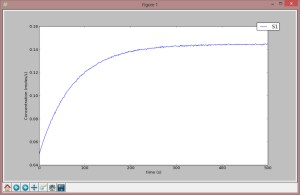
\includegraphics[width=220mm]{Minimization.jpg}
\caption{Output for the LMFit python example script discussed above.}
\label{fig:lmfitFig}
\end{sidewaysfigure}






